% Dissertation template for the Geophysics programs of the University of
% Liverpool.
%
% This document sets the configuration and assembles the individual chapters
% (stored in separate .tex files). See the declaration.tex file for
% instructions on including scanned signature.

% Fill these in and they will be set throughout the document
\newcommand{\Name}{Yoür Name}  % Note that you can use any Unicode character
\newcommand{\Degree}{Bachelor of Science in the subject of Geophysics (Geology)}
\newcommand{\Title}{Title of the dissertation}

\documentclass[11pt,a4paper,oneside]{book}
% Full Unicode support for non-ASCII characters
\usepackage[utf8]{inputenc}
% Typographical rules for English
\usepackage[english]{babel}
% Handling figures in PNG, JPG, PDF, etc
\usepackage{graphicx}
% Better and more extensive maths
\usepackage{amsmath}
% Set the borders of the page
\usepackage[width=150mm,top=40mm,bottom=30mm,headsep=10mm,headheight=5mm]{geometry}
% Include links and metadata in PDFs
\usepackage[pdftex,colorlinks=true]{hyperref}
% Define command to insert month name and year as date
\usepackage{datetime}
% Nice styling for headers and footers
\usepackage{fancyhdr}
% To control the style of section titles
\usepackage{titlesec}
% Add the bibliography to the table of contents
\usepackage[nottoc,chapter]{tocbibind}
% Formatting the bibliography
\usepackage[round]{natbib}
% To insert dummy text into this template. Can be removed.
\usepackage{lipsum}

% Define a date format that is just the month and year
\newdateformat{monthyear}{\monthname[\THEMONTH], \THEYEAR}

% Customize how Chapter headings are displayed
\titleformat{\chapter}[display]{\normalfont\bfseries\centering}{\vspace{-2cm}\LARGE Chapter \thechapter}{5pt}{\Huge}

% Setup metadata for the PDF and link colour
\hypersetup{
    pdftitle={\Title},
    pdfauthor={\Name},
    pdfsubject={Dissertation submitted for the degree of \Degree{}},
    linkcolor=black,
    citecolor=black,
    filecolor=black,
    urlcolor=blue
}

% Set fancy headers
\usepackage{fancyhdr}
\pagestyle{fancy}
\fancyhf{}
\lhead{\fontsize{10pt}{0}\selectfont\itshape \nouppercase\leftmark}
\chead{}
\rhead{\fontsize{9pt}{0}\selectfont \thepage}
\cfoot{}
\renewcommand{\headrulewidth}{0pt}
%\renewcommand{\chaptermark}[1]{\markboth{#1}{}}

% Increase the line spacing
\renewcommand{\baselinestretch}{1.5}

\begin{document}

  % Gather all of the .tex files for individual sections into a single
  % document. To add text and edit, open the individual files added with the
  % "\include{}" command.

  \pagestyle{plain}

  % You don't need to edit the cover, it will be generated from the variables
  % set at the very top of this document.
  % Cover page for the dissertation. Uses variables defined in the main
% dissertation.tex document. No need to edit things here.

%\addtolength{\topmargin}{-3in}

\thispagestyle{empty}

\begin{figure}[t!]
  \begin{center}
    
\includegraphics[width=0.7\textwidth]{figures/university-of-liverpool-logo.eps}
  \end{center}
\end{figure}

\vspace*{3cm}

\begin{center}
  \textbf{\LARGE \Title{}}
  \\[10mm]
  {\Large by}
  \\[10mm]
  {\Large \Name}
  \\
  \vfill
  \begin{minipage}[t]{0.7\textwidth}
    A dissertation submitted to the
    Department of Earth, Ocean, and
    Ecological Sciences,
    University of Liverpool, in partial fulfilment of
    the requirements for the degree of
    \Degree{}.
  \end{minipage}
  \\[3cm]
  \monthyear\today
\end{center}


  \frontmatter

  % You need to edit the declaration to include an image of your signature. See
  % the declaration.tex file for instructions.
  % Official declaration page that is required. The date is automatically set
% when the PDF is generated. Place a PNG file of your signature in the
% "figures" folder called "signature.png" (this exact name!). DON'T ADD THIS TO
% THE GIT RESPOSITORY!

\section*{Declaration}

\vspace{10mm}

I, \Name{}, confirm that the work submitted in this dissertation is my own, and
that appropriate credit has been given where reference is made to the work of
others.
\\[8mm]
\noindent Signature:

% To add your signature, place the "signature.png" file in the "figures"
% folder and uncomment the line below (remove the leading %).

\begin{figure}[h]
  %\includegraphics[width=50mm]{figures/signature.png}
\end{figure}

\noindent Date: \today

\newpage


  \section*{Acknowledgements}

Thank people, institutions, etc.


  % Add your abstract to the "abstract.tex" file. DO THIS PART LAST. It's
  % easier to write the abstract in the end (and do a good job of it).
  \section*{Abstract}

Add your abstract here.


  % Table of contents and lists of figures and tables are automatically
  % generated (yay!)
  \tableofcontents
  \listoffigures
  \listoftables

  \pagestyle{fancy}

  \mainmatter

  % These are the actual chapters of your dissertation. Add your text, figures,
  % tables, etc to these .tex files.
  \chapter{Introduction}

YOUR INTRODUCTION. The citations and bibliography are automatically handled by
BibTeX and the \texttt{natbib} package. Place the bibliographic information for
the references in the \texttt{references.bib} file and then cite your
references in the text (see below). The References section will be generated
automatically. To get the bibliographic information for papers, use the
\url{https://www.doi2bib.org/} website (DOIs are unique identifiers for
scientific publications, datasets, etc; you can find them in the paper PDFs or
publisher websites).

This is how you make citations: in the text \cite{Parker1973} or with
parenthesis \citep{Parker1973}. See
\url{https://www.overleaf.com/learn/latex/Natbib_citation_styles} for more
information.

The following is just filler text.

\lipsum[1-10]

  \chapter{Data and Methodology}

Section about your data and the methods used.


\section{Figures}

Figures are also automatically placed and numbered. You can reference them in
the text automatically as well (see Figure~\ref{fig:example}).

\begin{figure}[h]
  \begin{center}
    % Width can be set to particular size (10cm) or relative to the page size,
    % like 0.5\textwidth (for half page) or \textwidth (for full page).
    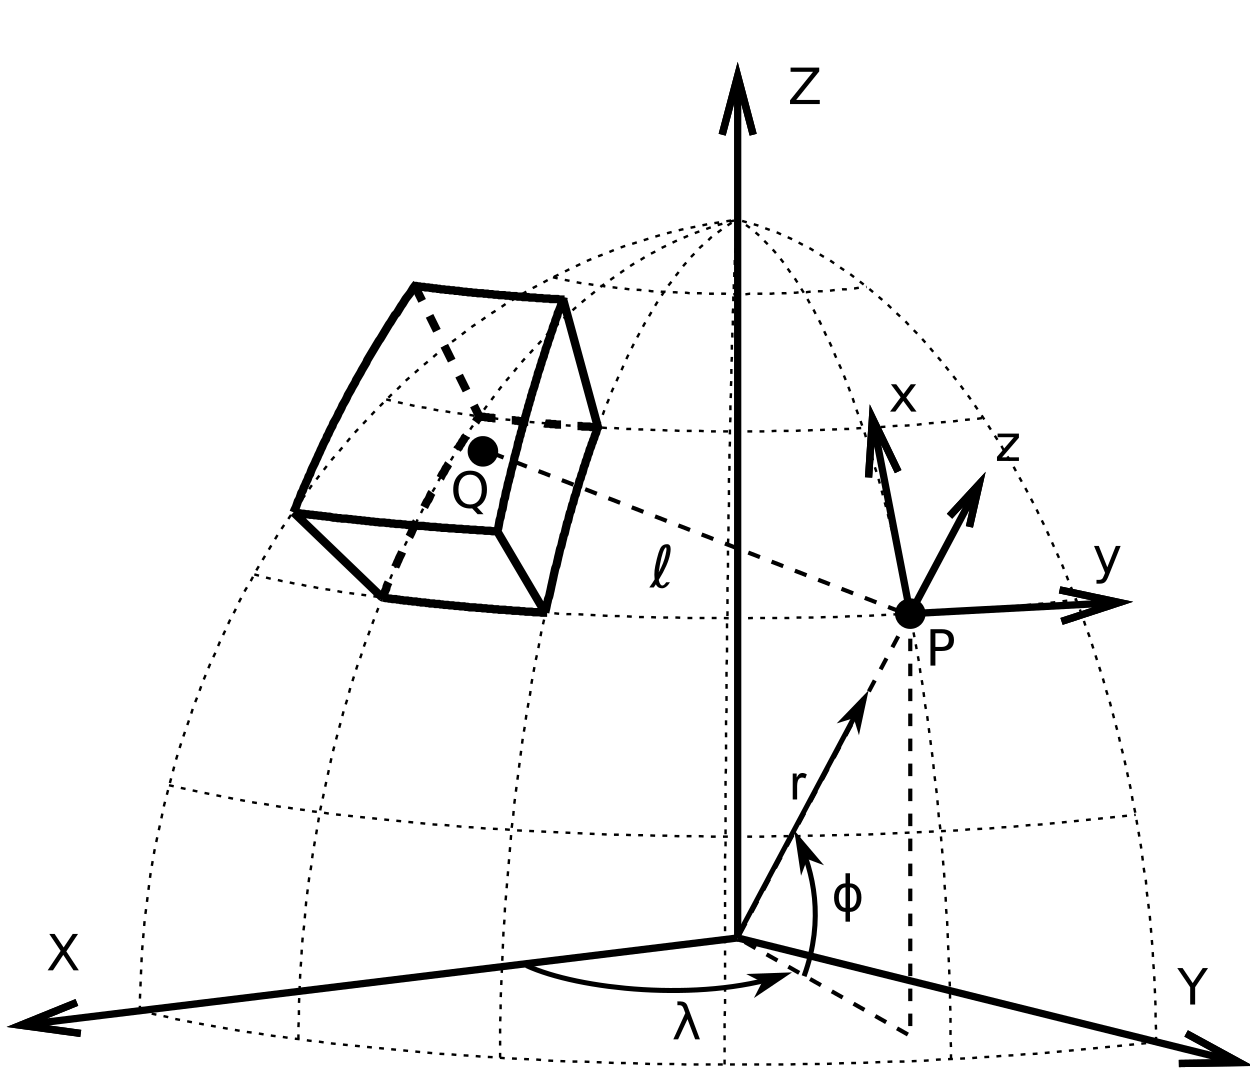
\includegraphics[width=0.5\textwidth]{figures/tesseroid-coord-sys.png}
  \end{center}
  \caption{
    This is the figure caption. Notice that the figure number is inserted into
    the text automatically. After \citet{uieda2015}.
  }
  % Label used to reference the figure in the text.
  \label{fig:example}
\end{figure}


\section{Tables}

This is an example of a table (see Table~\ref{tab:example}).

\begin{table}[h]
  \begin{center}
    % Two columns, one right aligned (r) the other centered (c)
    \begin{tabular}{rc}
      \textbf{First column}    &     \textbf{Second column}
      \\
      \hline
      Some values here  &  Others here
      \\
      Math too $\gamma = 10\ m/s^2$  &  Or not
    \end{tabular}
  \end{center}
  \caption{
    This is the table caption. Notice that the table number is inserted into
    the text automatically.
  }
  \label{tab:example}
\end{table}


\section{Equations}

This is how you can type out equations and reference them in the text. For
example, see Equation~\ref{eq:linear_least_squares} below.

\begin{equation}
  \mathbf{\hat{p}} =
    \left(\mathbf{A}^T\mathbf{A}\right)^{-1}
    \mathbf{A}^T\mathbf{d^o}
  % Label used to reference the equation in the text.
  \label{eq:linear_least_squares}
\end{equation}

  \chapter{Results and Discussion}

This is where you present the results and discuss their meaning.

  \chapter{Summary}

Conclusion of your dissertation. Summarize what was learned and why it's
relevant.

  \chapter{Future Work}

Look to the future. What would you do if you had another year?


  \pagestyle{plain}

  % Use the American Geophysical Union citation style
  \bibliographystyle{agu}
  % Use References instead of Bibliography (the default)
  \renewcommand{\bibname}{References}
  % The References section is automatically populated from the cited entries of
  % the references.bib file
  \bibliography{references}

  % If you want to have an appendix, uncomment these two lines and add an
  % appendix.tex file with the text. Sections declared in it will automatically
  % be numbered differently.

  %\appendix
  %\chapter{Appendix}

In order to create the plots and calculate results for this project we had to produce code through python language software in Jupyter lab. The repositories used were saved into the Github page Computer-Oriented Geoscience Lab ``compgeolab'' with the ones which provided all data presented named and described below:
\\ \footnotesize
\\
data/MarsTopo719.shape - Topography data file \\
data/gmm3\_120\_sha.tab - Gravity data file\\
environment.yml -directory that contains the collection of conda packages installed \\
prepare-gravity-grids.ipynb - Code required in order to export the now usable grids to a netCDF file \\
functions.py - Contains the utility functions for this project \\
mars-bouguer-density.ipynb - Code used to performed the calculations plotting figures for all regions used \\
Further-analysed-density.ipynb - Code used for plotting the figures whch were further analysed \\

\normalsize In order to test our code to see if the calculations would acquire an accurate density value we recreated the results of Carartori Tontini [2007]. 
\begin{figure}[H]
	\centering
	\subfloat{\includegraphics[width=65mm]{Figures/Caratori Tontini Recreation}\label{fig:C T recreation}}
	\subfloat{\includegraphics[width=71mm]{Figures/Density from Caratori Tontini}\label{fig:Density from C T}}
\end{figure}
The plots created obtained density value of $2300 kg/m^3$. This is slightly less than the $2400 kg/m^3$ from the paper but, this could be a consequence of using our gravity grid at a height of 10 km instead of 0 km. Despite that it does represent that to calculation performed in the code is successful in finding an accurate optimal Bouguer density; therefore, we can have confidence in the results shown in this Thesis.


\end{document}
